\part{Experimental Evaluation}
    \chapter*{Overview}
        Several different tests have been executed to assess the quality of the migration.
        
        I decided to focus on two main aspects:
        \begin{itemize}
            \item Data Quality
            \item Performance
        \end{itemize}
        
        \textbf{Data quality} is the most important requirement asked by Axpo: the accuracy of their business choices is strictly dependant on the quality of the data they are working with.
        
        \textbf{Performance} is also a very important factors, since several critical business processes need to access data in short amounts of time.\newline
        
        This part will describe how each test has been carried out, as well as the results obtained.\\
        Some problems encountered when assessing data quality or performances will also be discussed, as well as their impact on the testing phase.
        
    \chapter{Data Quality Tests}
        \label{section:tests:data}
Several tests have been performed on the Data Warehouse to assess the correctness of the data stored in it.

\section{Test Types}
    \subsection{Range Tests}
    This kind of test asserts that each database has data related to the same date range.

    The minimum and maximum dates for each table are extracted from each database and compared.
    Results are acceptable if the Data Warehouse contains at least the whole range present in the on-premise database.
    
    These tests initially recovered the date range over the whole dataset, but were later modified to retrieve more detailed information, computing the total number of hours\footnote{
        The number of hours is an important metric since most data are timeseries at hourly granularity.
        If the hour count is equal to the actual number of hours in a given time period, it means there are no ``holes'' in the dataset.
        These missing values could not be noticed with the initial test.
    } downloaded for each category\footnote{
        With \textit{category}, we mean all the relevant attributes needed to distinguish between two different values.
        This is important especially for forecasts, since multiple publications of the same hour must count as one (since the last value is always the most accurate).
    }.
    
    \paragraph{Exceptions}
        It is necessary to analyse all the results manually, since several exceptions can be made for the above rule.
    
        \subpar{Very old data}
            One possible exception is that of very old data.
            Some information related to several years ago are not currently used by the company and as such are not strictly necessary.
            
            Moreover, it may be currently impossible to retrieve these information from their providers, since they may no longer be accessible.
            
            On the other hand, if these information are needed it may be possible to perform a one-time manual data import from the on-premise database to the Data Warehouse.
            
        \subpar{Scheduling}
            If a table contains all data required except for the current day (or the next day in case of forecasts) it may be a problem related to the scheduling chosen for downloading data.
            
            For instance, the on-premise database may download data in the morning while the Data Warehouse downloads the same information during the afternoon.
            These test are thus dependent on the time they are executed.
            To avoid this limitation, the last two days are not taken into account when performing these tests.
            
        \subpar{Company needs}
            The most discerning element is, as always, the actual needs of the company.
            
            For example, if only the last year of some type of data is actually used, it is irrelevant if the on-premise database stores more years than the Data Warehouse, as long as the latter has the range required by the company.
    
    \paragraph{Failure}
        In case of failure, if no exceptions can be made for the data, Reply is notified and tasked with solving the issue.
        
        Solutions are specific to the kind of data of the provider.
        In some cases they may be as simple as changing a few parameters in the history retrieval settings, while in other cases, they may require more complex interactions and analyses of the provider, as well as additional development of the ETL procedures.
    
\subsection{Key Tests}
    This kind of test asserts that each database contains data related to the same information.
    
    It is a comparison based on the keys which identify a specific datum.
    Specific queries extract all the keys from each table in both databases and compare them.
    
    The most basic comparison is to perform an intersection between the two key datasets and count the number of obtained elements.
    This number, compared to the element count in the on-premise database, gives us a percentage of how many rows are in common between the two databases.
    
    More advanced tests are done manually, since they require in-depth knowledge of the domain, and are used to adjust the queries used to extract the keys.
    
    For example, it is sometimes necessary to aggregate or deaggregate some data, to use particular remappings or to rename some values (for instance, some values may be written all uppercase in a database and camel-case in the other; in other cases there may be additional characters, such as underscores).
    
    \paragraph{Exceptions}
        Usually the tests are repeated until all the data in the on-premise database is present in the Data Warehouse.
        
        However, depending on the company needs, it may be enough to settle for a lower value, depending on how the data are actually used.
    
    \paragraph{Failure}
        In case of test failure, Reply is notified with the problems encountered and will provide a fix.
        These tests will then be repeated until all keys are correctly present in both databases.
        
\subsection{Value Tests}
    The last kind of tests asserts that the two databases not only contain data related to the same information, but that they also contain the same data.
    
    This test is similar to a Key Test, but takes also into account the values associated with each key set.
    This kind of tests is able to expose problems related for example to wrong aggregation or deaggregation operations.
    
    The tests are considered successfully passed if we obtain the same common data percentage as the final results of the Key Tests (which is usually 100\%, unless it has been decided a lower value is enough for the company needs).
    
    \paragraph{Failure}
        In case of failure, Axpo and Reply work together to understand the cause of the problem.
        
        This collaboration is necessary since Axpo can provide technical domain information, while Reply has more knowledge related to the ETL process.
        Once the problem is identified, Reply will provide a fix.
        
        These tests will be then run again, until no further problems are found.

    
\section{Testing Suite}
    Each test needs to join together results obtained from different databases.

This operation is not trivial, since a query cannot be directly performed across multiple databases.

The solution I opted for was creating a script on Databricks, from which each database can be queried independently, the results can be put together and additional operations can be performed.

\subsection{Why Databricks?}
   The test suite has been developed on Databricks for several reasons.
    
    \paragraph{Already accessible}
        First of all, this environment was already accessible, since it has been used for the ETL process.
        Using an existing environment requires little to no additional configuration, and its costs are already included in the project budget.
    
    \paragraph{Multiple languages}
        Secondly, Databricks supports multiple languages in the same workbook.
        The query results have been merged using Python, while additional analyses have been performed on the resulting dataset in SQL, taking full advantage of the strengths of both language.
    
    \paragraph{Spark}
        A third important aspect is that Databricks natively supports Spark, meaning that each database could be queried at the same time.
        Moreover, each query is automatically parallelized to further improve their performance.
    
\subsection{Script Description}
    \begin{figure}
        \centering
        \begin{subfigure}{\textwidth}
            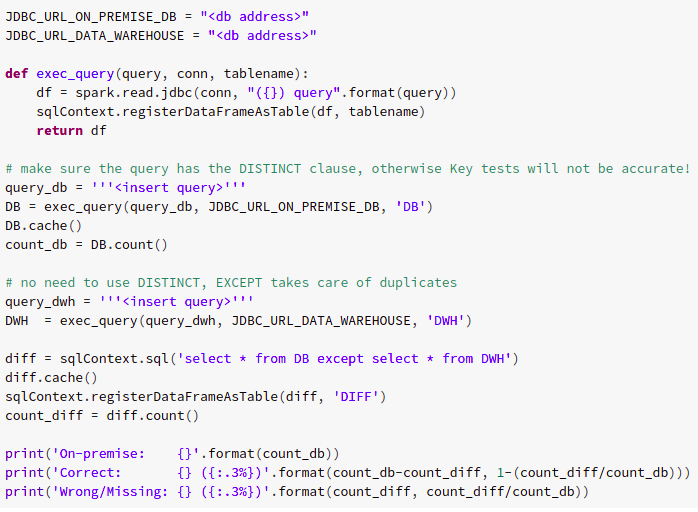
\includegraphics[width=\textwidth]{res/tests/test_suite.png}
            \subcaption{Python}
        \end{subfigure}
        
        \begin{subfigure}{.3\textwidth}
            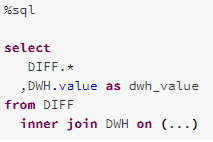
\includegraphics[width=\textwidth]{res/tests/test_suite_sql.png}
            \subcaption{SQL}
            \label{fig:tests:data:suite:sql}
        \end{subfigure}
        
        \caption{Testing suite.}
        \label{fig:tests:data:suite}
    \end{figure}

    The script created, shown in Figure \ref{fig:tests:data:suite}, requires as input two queries.
    
    The first query will be performed on the on-premise database, while the second on the Data Warehouse.
    These queries must return data in the same format, since the results are going to be merged.
    
    By using Spark, the scripts performs a join between both results, taking all values from the on-premise database which have not been found in the Data Warehouse.
    
    From this new dataset it is possible to compute the data match percentage between the two databases.
    
    \paragraph{SQL}
        A separate cell, using SQL, allows users to perform \textit{ad-hoc} queries on the mismatching values, which has been used abundantly to analyze the problems found.
        
        For example, the query shown in \ref{fig:tests:data:suite:sql} compares the values stored in each database, excluding the rows which are present only in the local database.
        This query proved to be extremely useful for understanding issues related to Value tests.

\section{Test Results}
    Several tests have been executed on the Data Warehouse.

Each time, the testing suite has been modified to increase the result accuracy.

\subsection{Preliminary Results}
    Preliminary tests have shown many problems related with the ETL process.

\paragraph{Range tests}
    Range tests have shown that 50\% of the data streams on the Data Warehouse have at least the same date range than the on-premise databases.
    
    Out of 38 tests executed, we had the following results:
    \begin{itemize}
        \item 17 data streams had a greater date range on the Data Warehouse than on the on-premise databases.
        \item 2 data streams had the same range on both databases.
        \item 16 data streams on the Data Warehouse had a smaller date range compared to the local databases.
        \item 3 Data Warehouse data streams were empty
    \end{itemize}

\paragraph{Key tests}
    Key Tests results were more disappointing at first.
    Out of 38 possible tests, we were able to perform only 16.
    The other tests could not be written because there were information (for example, columns or remapping tables) missing.
    
    Out of these 16 tests, only two initially gave acceptable results, with 98\% and 92\% of the data contained in the on-premise database being available on the Data Warehouse.
    All the other results were pretty low, with 5 of them around 30\%, 2 lower than 10\% and the remaining 8 at 0\%.
    
\paragraph{Further analysis}
    These results, especially the ones at 0\% meant it was necessary to further analyze the situation, to understand if the issue laid within the Data Warehouse or the testing suite itself.
    
    We began exploring both databases manually, with the support of Axpo domain specialists.
    Several differences in the data formats had been found.
    For example, some fields contained manually generated data, while in other cases an hour notation different from the standard format was used in the on-premise databases.
    In some other cases, the data was supposed to be different, so this kind of test could not be applied (see section \ref{section:tests:data:fct_publ} for details).
    
    This lead to an improvement of the testing suite, now taking into account these differences.



\subsection{Test Suite Improvements}
    After some improvements in the test suite, the tests were then executed again, since the first results were proven not to be representative of the Data Warehouse quality.

\paragraph{Range tests}
    Range tests were changed to obtain more detailed information.
    Overall, the results obtained were very similar to the previous ones, but a few additional issues were discovered.
    
    For example, we noticed that in some cases date ranges varied depending not only on the provider, but also on the country for the same provider.
    
    These results indicated that some problems were related only to particular cases of the ETL process.

\paragraph{Key tests}
    Key tests results became much more promising, meaning that the main problem didn't reside in the Data Warehouse but in the testing suite itself.
    
    Out of the initial 16 tests, we obtained a much higher consistency level, as shown in Figure \ref{fig:tests:data:hist_1}.
    
    \begin{figure}
        \centering
        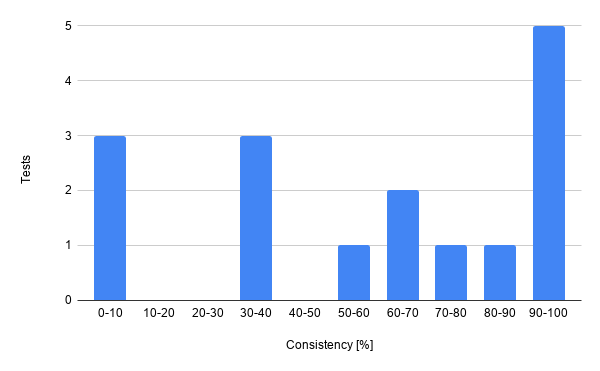
\includegraphics[width=\textwidth]{res/tests/data_hist_1.png}
        \caption{Consistency level histogram on key tests.}
        \label{fig:tests:data:hist_1}
    \end{figure}
    
    A high number of tests were successful, with 3 tests having an accuracy greater than 99\%.
    A value of 100\% is very difficult to achieve, since the data in the on-premise databases is downloaded at a different moment than that on the Data Warehouse.
    This difference can produce some false negative results, but they will always be related to a single day (usually the current one).
    As such, a value greater than 99\% can be considered an acceptable threshold.
    
    It was also shown that there were some inconsistencies between the two databases, but we were also able to identify their cause.
    Two tests failed because the required information had not been downloaded at all, one because hours had been remapped incorrectly, while the other failures were caused by a smaller date range.
    
    In the first case, the on-premise database contained information about specific countries or models, while the Data Warehouse contained information about different countries or models.
    This issue can usually be solved by a simple change in the downloader configuration.
    
    The two other problems were equally easy to solve.
    For the remappings, it was necessary to fix some values in the remapping table and rerun the procedure to materialize the correct values, while for the data range it was required to change the downloader configuration.
    
\paragraph{Value tests}
    Considering the acceptable results obtained with the Key tests, we decided to assess the correctness of the values.
    Out of 16 queries, 7 were related to forecasts, for which this kind of tests could not be applied.
    As a consequence, only the remaining 9 tests have been executed.
    
    \begin{figure}
        \centering
        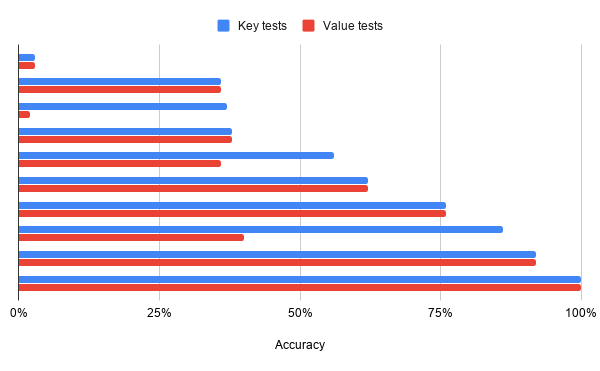
\includegraphics[width=\textwidth]{res/tests/data_val_1.png}
        \caption{Key-Value test results.}
        \label{fig:tests:data:value_1}
    \end{figure}
    
    The results, as shown in Figure \ref{fig:tests:data:value_1} were very positive, with 6 tests (66\% of the testing suite) having 100\% accuracy, while the others gave respectively 64\%, 47\% and 5\%.
    
    It should also be noted that in some cases the values stored in the on-premise databases were wrong, while those present in the Data Warehouse were correct.
    In these cases, it is impossible to perform an accurate analysis, and lower values are also accepted.
    This process is however carried out manually and these kind of exceptions are made for specific cases after a careful analysis.
    
\subsection{ETL Fixes}
    The identified issues have been communicated to Reply, along with examples of incorrect values.

At the time of writing, Reply has only fixed issues related to Value tests, meaning that the overall data quality is still going to improve with time.

\begin{figure}
    \centering
    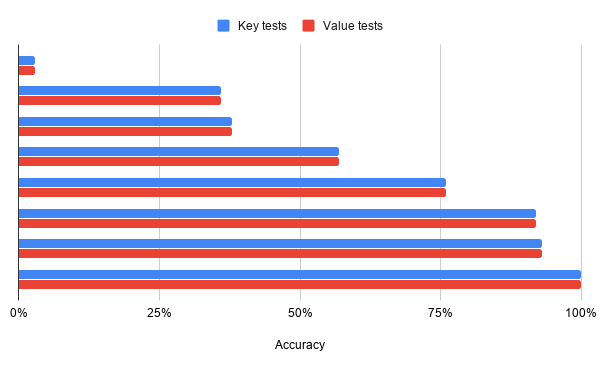
\includegraphics[width=\textwidth]{res/tests/data_val_2.png}
    \caption{Key-Value tests after Reply fixes.}
    \label{fig:tests:data:results_3}
\end{figure}

The tests have been executed once more, obtaining excellent results, as shown in Figure \ref{fig:tests:data:results_3}.

We can see that each Value test has the same accuracy level as their respective Key test.
Value tests, on the other hand are still incomplete.

From these results, we can understand that the ETL process is not yet able to download all the required data, but each downloaded information is correct.

    
\subsection{Conclusions}
    The results discussed above show that the ETL process, once properly tuned, is effective at downloading data and that the downloaded information are correct.

Some problems, however, are still present in the Data Warehouse, which, once fixed, will certainly increase the results of the tests.

It has been shown that building a proper testing suite is a very complex matter, and a poorly constructed one can prove ineffective at detecting issues either by giving false negative or false positive results.

\paragraph{False negatives}
    A false negative result happens when a given datum appears to be different from the on-premise database but in reality is correct.
    This can happen for two main reasons.
    
    In some cases, values have been processed in the on-premise database, but this process has not been replicated correctly by the test.
    In this case, it is necessary to apply the same kind of data transformation in the test.
    
    Another possible scenario is caused by a different handling on \texttt{NULL} values.
    For example, some coefficients for specific hours are sometimes not specified by the providers.
    The Data Warehouse stored these missing values as \texttt{NULL}s, while in the on-premise database they were assigned default values, which were different depending on the type of coefficient.
    
\paragraph{False positives}
    A test can also produce false positive results, especially if the test is too much generic.
    These results can hide existing problems in the Data Warehouse, showing that there are no problems.
    
    For example, let us consider a table containing information about multiple countries.
    Let us also assume that for Austria we have data ranging from 2015 to 2019, while for Germany (for which we should have the same range) we are missing data related to 2019.
    
    A generic test, computing the minimum and maximum date ranges across all data would show a range of 2015-2019, which means that there are no problems.
    This result is, however, a false positive.
    A more in-depth test, testing the minimum and maximum date ranges for each country would however notice the issue.
    
    Most tests are however more complex than this example however, since it is necessary to aggregate information across a large number of dimensions.
    
    


    
\section{Problems}
    Several problems have been encountered as a result of the tests carried out.
After each problem has been solved, we executed the tests once again, obtaining better results.
Perfect results have not been achieved yet, meaning that more problems need to identified and solved.
The results obtained are however enough to show the effectiveness of the testing suite.

This section will provide a description of the main problems identified.

\subsection{Pivoting}
    In some cases, tables on the on-premise database are pivoted differently than those on the Data Warehouse.
    
    If the company requires a specific output format the table on the Data Warehouse will be unpivoted accordingly, meaning that it will then be possible to run the tests on the new table.
    On the other hand, if both formats are acceptable and no unpivoting operation is to be performed, it is impossible to execute Key and Value Tests, since the structures are too much different.
    
    In this case a few manual tests will be executed to assert at least a degree of correctness, even though a comprehensive testing suite has not been developed.

\subsection{Forecast Publications} \label{section:tests:data:fct_publ}
    Forecasts are very difficult to compare.
    
    The values downloaded from a provider are the results of a specific run of a certain algorithm.
    Different runs usually give different results, since the input data is different.
    Moreover, these algorithms are proprietary, so it isn't possible to investigate their behaviour.
    
    Forecasts are published multiple times a day.
    Depending on when the data is downloaded, different values are obtained.
    
    The main problem arises from different download schedules between the on-premise tools and the ETL processes developed by Reply.
    Different download schedules mean different values obtained, which invalidate most tests.
    As a consequence, this kind of data can only be tested on download ranges.
    Additional tests have to be performed by domain experts during real data application scenarios (i.e., running a tool with the new data and manually seeing how well it performs).
    
\subsection{Floating Points}
    Floating point values present some limitations when performing comparisons.
    This kind of data is by design approximate, meaning that it won't store the exact value but an approximation of it \cite{bib:tests:float_intersect}.
    
    This is not usually an issue, since the approximation is extremely close to the actual value, but it can present some problems when performing equality checks, since they are based on exact values.
    In this case, values which may appear to be the same are considered different, resulting in wrong metrics.
    
    The solution is to convert all floating point values to the \code{DECIMAL} data type, which can support a specified number of decimal digits.
    
    Decimal data types are stored differently from floating points, the latter being based on a value multiplied by an exponent, while the former being just a plain representation of the number, with the possibility of specifying how many digit are decimal.
    
    Since decimal data types represent exactly all the digits in the number, operations such as equality checks and intersections (which internally rely on equality checks) can be performed without fear of getting wrong results.

\subsection{Different Values}
    In multiple cases, Key tests indicated a high consistency level but Value tests gave poor results.
    
    I analyzed each issue with the help of Reply and identified the proper solution.
    A consistent number of problems was caused by operations applied on the data in the on-premise database.
    These operations were specific to the type of data, so there wasn't a unique or common solution.
    
    For example, I notice that the quantities of energy transferred between different zones were different, although all the keys were correct.
    This meant that the Data Warehouse contained the correct datum but with the wrong value, compared to the on-premise database.
    
    \paragraph{Website data}
        The first check we did after having identified the problem was controlling that the values present on the website were identical to those stored in the Data Warehouse.
        
        The website had two different categories of data, named \textit{Day Ahead} and \textit{Total}.
        The specifics given by Axpo indicated that the value to download was \textit{Total}.
        
        We compared these value with the results obtained from the Value test and noticed that the data in Data Warehouse was correct, while the on-premise database contained different numbers.
    
    \paragraph{Data operations}
        After having identified this problem, I asked the Axpo specialist who used this kind of data if the local database performed some operations on the data.
        It turned out that the quantities stored in the on-premise database were the net transferred amount and not the whole amount.
        
        Table \ref{tab:tests:data:operations} shows the difference between whole and net transfers amount.
        In the first case, we record how much energy each zone has transferred, while in the second we only store the difference between the two values.
        This behaviour has been replicated in the Value test.
        
        \begin{table}
            \centering
            \begin{tabular}{|c|c c c|}
                \toprule
                Amount                 & From & To & Quantity \\
                \midrule
                \multirow{2}{*}{Whole} & A    & B  & 100      \\
                {}                     & B    & A  & 35       \\
                \midrule
                \multirow{2}{*}{Net}   & A    & B  & 65       \\
                {}                     & B    & A  & 0        \\
                \bottomrule
            \end{tabular}
            \caption{Whole vs net energy transfer amounts between zones.}
            \label{tab:tests:data:operations}
        \end{table}
        
        
        
    \paragraph{Different data stream}
        Even with this normalization operations in place, the Value test was still indicating the presence of several errors.
        
        While comparing the newly computed results obtained from the test with the provider's website, we noticed that the values of the on-premise database matched the \textit{Day Ahead} column from the website.
        
        This problem has been presented to Axpo, and we understood it was necessary to change the initial requirements, adding this kind of data to the original planning.






    \chapter{Performance Tests}
        Multiple tests have been performed to assess the performance of the Data Warehouse, comparing it with the on-premise databases. 

\section{Test Types}
    \subsection{Metrics}
    The first approach has been to analyze some metrics internal to the database.

These metrics are automatically managed by the database itself and show a huge variety of information about the current configuration of the database.

\paragraph{Dynamic Management Views}
    In SQL Server, Dynamic Management Views (\textit{DMVs}) are system views which return server state information useful for monitoring the health of a server instance, diagnosing problems and tuning performance.
    
    The amount of information shown is huge (several thousands of metrics), but only a few have been useful for the performance analyses I carried out.
    
\paragraph{Other metrics}
    Most metrics are related to advanced aspects (e.g. the number of locks performed per second or the number of pages for the whole database) which have proved not to be useful for the performance analyses.
    
    These metrics are indeed used for an in-depth analysis or for advanced tuning of the Data Warehouse.
    
    In my case, however, I wanted to show the difference in query execution times, since it is the most relevant aspect for Axpo employees.

\subsubsection{Metrics Analyzed}
    One of the most important metric analyzed is the execution time of each query submitted to the database.
    
    This value can be retrieved by querying the DMV \texttt{sys.dm\_exec\_query\_stats} \cite{bib:tests:perf:dmv_doc}.
    
    A lot of information are available, such as:
    \begin{itemize}
        \item The query itself.
        \item The execution plan chosen for the query.
        \item How many times the query has been executed.
        \item Execution time.
        \item Physical / Logical reads performed.
        \item Physical / Logical writes performed.
        \item Time used to compile the execution plan.
        \item Memory used to compile the execution plan.
        \item Degree of parallelism (\textit{DOP}).
    \end{itemize}
    
    The only information I decided to analyze is the execution time, since the other were too much specific and low-level.
        
    \paragraph{Values available}
        There are four different values related to execution time:
            \begin{itemize}
                \item Last elapsed time.
                \item Total elapsed time.
                \item Last worker time.
                \item Total worker time.
            \end{itemize}
            
        The first two refer to the total time used for executing the query, while the other are specific to CPU usage.
        
        Both these values are important, since we can compare CPU time to the total elapsed time to understand the impact of locks.
    
    \paragraph{Complications}
        There are however a few complications in this computation.
        
        First of all, if the query has been parallelized (DOP $>$ 1) worker times are aggregated \cite{bib:tests:perf:dmv_time}.
        As a consequence, it is necessary to divide this value by the DOP.
        
        Secondly, all total values need to be divided by the execution count, since we need to compare the execution times independently of how many times a query has been called.
        These values are however stored as integers (without any decimal digits), so they all need to be converted to a decimal type, otherwise we would lose information about decimal digits.
        
        Lastly, values are expressed in microseconds (even though they are accurate up to milliseconds \cite{bib:tests:perf:dmv_doc}).
        These values have been converted to seconds to provide better readability.
        
    \paragraph{Query}
    
        \begin{figure}
            \centering
            \begin{subfigure}{\textwidth}
                \fbox{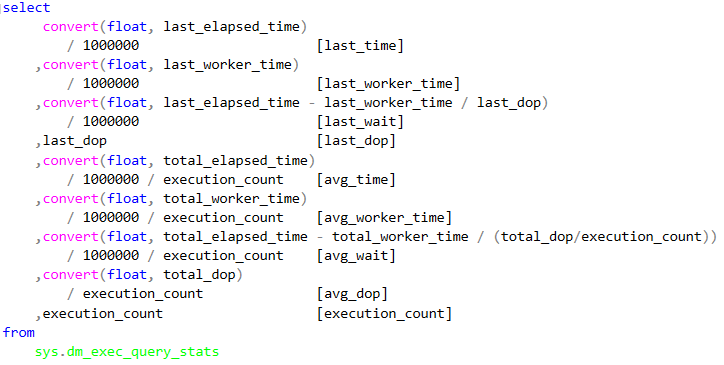
\includegraphics[width=\textwidth]{res/tests/metrics_exec_time_detailed.png}}
                \subcaption{Detailed information.}
                \label{fig:tests:perf:queries:detailed}
            \end{subfigure}
            
            \begin{subfigure}{\textwidth}
                \fbox{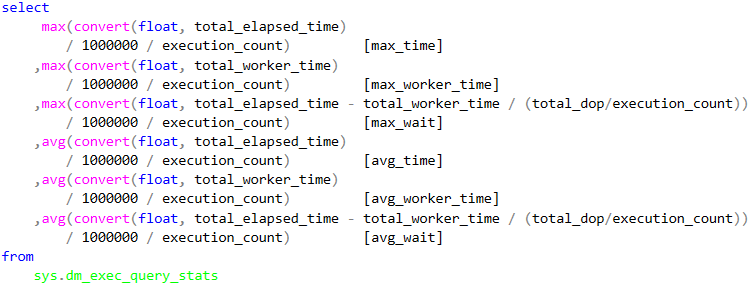
\includegraphics[width=\textwidth]{res/tests/metrics_exec_time_aggregated.png}}
                \subcaption{Average and max metrics.}
                \label{fig:tests:perf:queries:aggregated}
            \end{subfigure}
            
            \caption{Queries used for analyzing query execution times.}
        \end{figure}
        
        Two different queries have been used, as shown in figures \ref{fig:tests:perf:queries:detailed} and \ref{fig:tests:perf:queries:aggregated}.
        The first query produces a detailed output of the execution of each query, while the second shows average and peak execution times across all queries.
        
        \subpar{Aggregate information}
            Aggregate information give a quick but effective overview of the database.
            
            Maximum values show the worst case scenarios, while average values are representative of the database performance.
            We can also understand if there is a problem with locking by comparing elapsed and waiting times.
            If the two values are close, it means that most time was spent waiting.
        
        \subpar{Detailed information}
            Detailed information allow to analyze each query independently.
            
            By ordering the results in descending order, we can easily find how many queries present problems (such as high wait times) or are computationally heavy (which could mean they are not optimized).
            By showing an additional field, called \texttt{sql\_handle}, a unique identifier for that query can be obtained.
            By joining this value with other DMVs, it is possible to perform additional analyses on that specific query.
            
            Last execution times are also shown, since they could differ from average times.
            A large difference can imply there are moments in which the database is under a heavy load and performs poorly.
\subsection{Queries}
    Several generic queries have also been executed on both the Data Warehouse and the on-premise databases.
These queries present different properties, and are representative of the actual workload.

The execution times of these queries have been recorded and compared.

\subsubsection{Query types}
    Specific queries have been developed to test different usage scenarios.
    
    These queries are:
    \paragraph{Count}
        This query needs to count how many rows are in a table.
        It requires a scan of the whole table, but access to no values.
    
    \paragraph{Generic selection}
        This query is expected to perform a sequential scan of the table and return all values.
        The speed of this query depends solely on the database power.
        
    \paragraph{Low selectivity}
        This query has a simple \code{WHERE} clause, which is expected to retrieve around 50\% of the data.
        
    \paragraph{High selectivity}
        This query has a more complex \code{WHERE} clause ranging over multiple attributes.
        It is expected to retrieve a small amount of data.
        
    \paragraph{Ordering}
        This query retrieves a medium-sized dataset and is tasked with sorting it according to a given value.
        
    \paragraph{Aggregation}
        This test divides the data into groups and computes an aggregated value for each group.
        
    \paragraph{Duplicate removal}
        This query selects a large number of rows and tries to remove all duplicate from multiple columns.
        
    \paragraph{Insertion / Deletion}
        Two similar queries insert a medium amount of rows in a table and then remove them.
        Times are recorded independently for insertion and deletion.
        
\subsubsection{Table types}
    \textit{Azure SQL Data Warehouse} supports three different table types, offering different indexing options \cite{bib:tests:perf:indexing}.
    
    Tests have been carried out on all three types, to serve both as a comparison between different options and to give a more precise estimation of the improvements provided by the Data Warehouse.
    
    \paragraph{Heap tables}
        Heap tables are optimized for insertion and deletion operations.
        
        Rows are stored in the order in which they are inserted into the table, although the Database Engine can move data around in the heap to increase the storage efficiency \cite{bib:tests:perf:heap}.
        
        As a consequence, the data order cannot be predicted. Clustering indexes cannot be applied to heap tables.
        
    \paragraph{Column-store index tables}
        Column-store tables store data as columns, as opposed to the traditional row storage \cite{bib:tests:perf:columnstore}.
        
        This storage type allows very fast access to multiple rows of a single column, since they are stored in the same memory block.
        Additionally, only the selected columns are fetched, avoiding retrieval of unnecessary data.
        
        Column-store tables can be either clustered or non-clustered.
        The former allows specifying only a single clustering column.
        
    \paragraph{Clustered index tables}
        Clustered tables store data in sorted order, depending on the clustering index chosen.
        They are very efficient for retrieving sorted data and for performing selection operations on the cluster index.
        
        On the other hand, sorting operation of different attributes may be penalized, compared to other table type.
        Insertion and deletion operation need to update the clustering index each time, creating additional overhead.
        
\subsubsection{Setup}
    The queries have been executed on both databases on identical tables, having the both same structure and data.
    
    \paragraph{Measurements}
        \begin{figure}
            \centering
            \fbox{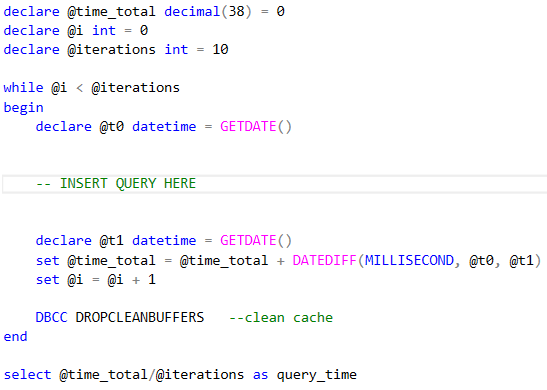
\includegraphics[width=.7\textwidth]{res/tests/sql_wrapper.png}}
            \caption{SQL wrapper for collecting accurate query execution time.}
            \label{fig:tests:perf:queries:wrapper}
        \end{figure}
    
        A small SQL wrapper for the query, shown in Figure \ref{fig:tests:perf:queries:wrapper}, has been created in order to collect accurate measurements.
        
        This wrapper records both the starting and ending time of the query, from which the actual execution time can be computed.
        
        Multiple executions of the same queries are performed in order to improve result accuracy.
        The resulting execution time is the average of all the times obtained.
        
    \paragraph{Caching}
        Databases can cache query results to speed up successive executions of the same query.
        
        Although caching improves query performance, it can produce misleading results in our tests, since we are going to execute the same query many times in a row.
        
        It is impossible to disable result caching for a specific query, but it is possible to clean up the whole cache, preventing it from invalidating test results.
        
\section{Test Results}
    \subsection{Metrics}
    This kind of tests has been performed on both the main on-premise database and the cloud Data Warehouse.

\subsubsection{Aggregated metrics}
    \begin{table}
        \centering
        \begin{tabular}{|c|r r r|r r r|}
            \toprule
            Database    & Max elapsed & Max CPU  & Max wait & Avg elapsed & Avg CPU & Avg wait \\
            \midrule  
            On-premise  & 3147.153    & 1108.736 & 3130.507 & 4.789       & 2.602   & 4.379    \\
            Cloud       &  150.743    &   48.563 &  126.462 & 0.342       & 0.115   & 0.269    \\
            \midrule  
            Proportion  & 4.79\%      & 4.38\%   & 4.04\%   & 7.14\%      & 4.43\%  & 6.13\%   \\
            \bottomrule
        \end{tabular}
        \caption{Aggregated query execution times metrics.}
        \label{tab:tests:perf:metrics:aggregated}
    \end{table}
    
    From the results of this test, shown in Table \ref{tab:tests:perf:metrics:aggregated}, we can see that the cloud Data Warehouse can produce, on average, query results in 7.14\% of the time required by the on-premise database (more than 12 times faster).
    Wait times are a bit smaller on the Data Warehouse (keeping in mind the proportion), but are not considerably reduced.
    
    More interestingly, the highest execution times recorded are smaller on the Data Warehouse by a large amount (around than 20 times lower).
    Average CPU times have similar proportions considering both the highest and the average values recorded.
    
    A more detailed analysis is however required before coming up to some conclusions.
    
\subsubsection{Detailed metrics}
    The metrics analyzed are shown in Tables \ref{tab:tests:perf:metrics:detailed:aa} and \ref{tab:tests:perf:metrics:detailed:dwh}.
    These tables contain only the ten queries with the highest total execution time.
    A larger number of queries, however, has been analyzed, even though they are not listed for readability purposes.

    One of the first things which can be noticed is that the last execution times on the on-premise database are often different from the average values (as expected, since they depend on the current database usage), while on the Data Warehouse the last execution times are, in most cases, identical to the average values.
    
    \paragraph{Execution Count}
        Upon analyzing the execution count for each query, it was noticed that on the Data Warehouse most queries had been executed just once.
        As a consequence, the average query execution count for both databases have been computed for both databases.
        
        The results showed that the Data Warehouse had not been used enough yet: each query had been executed on average 9 times, compared to an average of 5129 in the on-premise database.
        
    \paragraph {Data Warehouse Usage}
        Moreover, I knew that only a restricted subset of Axpo users where actively using the Data Warehouse, since the migration was still in development and the data needed by the other users had not been migrated yet.
        This smaller number of users meant that the average workload of the Data Warehouse was lower than in the on-premise database.
        
        Having a smaller workload, meant that the Data Warehouse could use more resources to compute the query results.
        
        As a result, we can conclude that these metrics can only provide a generic overview of the Data Warehouse performance at the current time.

\begin{table}[p]
    \centering
    \begin{tabular}{|r r r|r r r|c|}
        \toprule
        \multicolumn{3}{|c|}{Last execution} & \multicolumn{4}{c|}{Average values} \\
        \midrule
        Total       & CPU     & Wait         & Total    & CPU     & Wait     & DOP  \\
        \midrule
        6839.531    & 224.368 & 6820.834     & 3131.482 & 197.520 & 3115.022 & 12   \\
         718.741    & 163.319 &  555.421     &  718.741 & 163.319 &  555.421 &  1   \\
         484.972    &  99.821 &  385.151     &  484.972 &  99.821 &  385.151 &  1   \\
         272.092    & 186.531 &  256.547     &  258.351 & 165.731 &  244.540 & 12   \\
         210.750    &  94.374 &  202.885     &  210.750 &  94.374 &  202.885 & 12   \\
         266.322    &  64.247 &  202.074     &  266.322 &  64.247 &  202.074 &  1   \\
         247.747    &  52.608 &  195.138     &  247.747 &  52.608 &  195.138 &  1   \\
         250.279    & 466.570 &  211.398     &  221.347 & 425.721 &  185.870 & 12   \\
         183.070    &  42.352 &  140.717     &  183.070 &  42.352 &  140.717 &  1   \\
         148.721    & 120.985 &  138.639     &  111.562 & 108.767 &  102.498 & 12   \\
 \bottomrule
    \end{tabular}
    \caption{Detailed metrics for on-premise database.}
    \label{tab:tests:perf:metrics:detailed:aa}
\end{table}

\begin{table}[p]
    \centering
    \begin{tabular}{|r r r|r r r|c|}
\toprule
\multicolumn{3}{|c|}{Last execution} & \multicolumn{4}{c|}{Average values} \\
\midrule
Total       & CPU     & Wait         & Total    & CPU     & Wait     & DOP  \\
\midrule
150.742     & 48.562 & 126.461       & 150.742  & 48.562  & 126.461  & 2    \\
140.425     & 45.220 & 117.814       & 140.425  & 45.220  & 117.814  & 2    \\
134.712     & 35.646 & 116.889       & 134.712  & 35.646  & 116.889  & 2    \\
134.385     & 46.860 & 110.955       & 134.385  & 46.860  & 110.955  & 2    \\
120.121     & 37.765 & 101.238       & 120.121  & 37.765  & 101.238  & 2    \\
117.977     & 36.492 &  99.731       & 117.977  & 36.492  &  99.731  & 2    \\
114.978     & 34.205 &  97.875       & 114.978  & 34.205  &  97.875  & 2    \\
116.704     & 38.060 &  97.674       & 116.704  & 38.060  &  97.674  & 2    \\
115.938     & 37.497 &  97.189       & 115.938  & 37.497  &  97.189  & 2    \\
116.585     & 39.543 &  96.813       & 116.585  & 39.543  &  96.813  & 2    \\
 \bottomrule
    \end{tabular}
    \caption{Detailed metrics for Data Warehouse.}
    \label{tab:tests:perf:metrics:detailed:dwh}
\end{table}
    
\subsubsection{Problems}
    Tests on metrics, although properly structured, proved not to be representative of the Data Warehouse.
    
    \paragraph{Workload}
        The large difference in active usage caused the data to be too much influenced by noise, in the form of different workloads between the two databases.
        
        On the one hand, the local database was actively used by a large number of users, which meant that the database had to deal with a high amount of queries at the same time.
        
        On the other hand, the Data Warehouse was used by a restricted number of users, leaving more resources available for computing the results.
    
    \paragraph{Different queries}
        These metrics analyzed the execution times of all the queries executed on each database.
        It is important to keep in mind that the queries analyzed are not the same however.
        It is very likely that a consistent number of complex and computationally demanding queries has been run only in the on-premise database, since the Data Warehouse is newer and still incomplete.
        
        Some users, who usually execute complex queries, still haven't had the possibility of computing on the cloud, since the data they need hasn't been migrated yet.
        These queries will very likely increase the metrics obtained from the Data Warehouse.
        
\subsection{Queries}
    \subsubsection{Setup}
    This test has been performed on actual data used by Axpo.
    The view selected contains forecasts from multiple providers related to multiple categories.
    It has been chosen since it is one of the largest and slowest tables used by the company.
    The view contains 106 million rows.
    
    \paragraph{Materialization}
        Executing tests on a view would have produce inaccurate results, since multiple operations (mostly joins with dimensional table) are performed each time.
        To avoid this problem, the data has been copied to a separate table, created appositely for testing.
        
        In this way, we also made sure no one else would use this table while the tests were being executed.
        
    \paragraph{Excessive table size}
        The size of the table was still however excessive for some tests; the two main problems encountered were:
        \begin{itemize}
            \item Excessive computational times
            \item Not enough RAM to store the results
        \end{itemize}
        
        The first issue prevented running an appropriate number of tests, since a single query execution could take more than half a day.
        It was necessary to perform multiple runs of each query to obtain more reliable results, so each test would have taken several days.
        
        The second problem was related to the PC used for executing the tests: asking to retrieve a huge number of rows would have required a very large amount of RAM on the machine to temporarily store the results.
        Since the machine was limited to 8GB RAM, it often encountered \textit{Out of Memory} errors, which prevented the tests from completing.
        
        As a consequence, I decided to leave only the most recent 10 million records, and perform the tests on this smaller set.
        Since all data in the original table is updated daily, taking the last \textit{n} days leaves all the value distributions intact.
        
\subsubsection{Results}
    The execution times measured from the queries mostly confirmed the results obtained from the metrics.

    \begin{figure}[p]
        \centering
        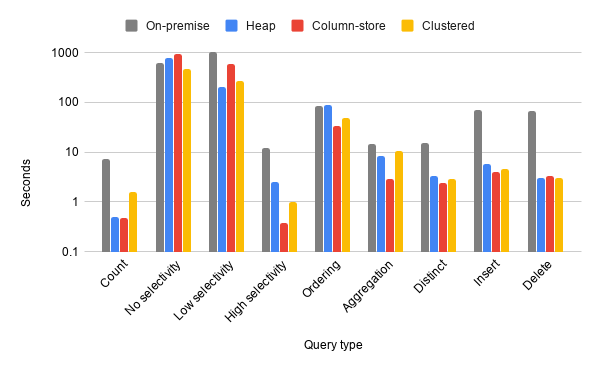
\includegraphics[width=\textwidth]{res/tests/perf_queries.png}
        \caption{Query execution times for both databases. Different table options have been tested.}
        \label{fig:tests:perf:queries:results}
    \end{figure}
    
    \begin{figure}[p]
        \centering
        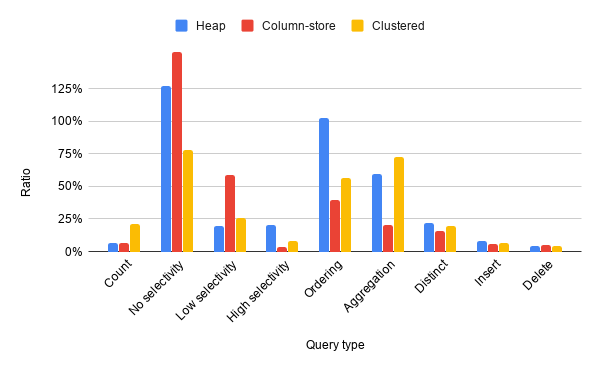
\includegraphics[width=\textwidth]{res/tests/perf_queries_perc.png}
        \caption{Execution time ratio between Data Warehouse and on-premise database, for each query type.}
        \label{fig:tests:perf:queries:results:ratio}
    \end{figure}
    
    The times obtained are shown in Figure \ref{fig:tests:perf:queries:results}.
    
    Figure \ref{fig:tests:perf:queries:results:ratio} shows the execution time ratio between the Data Warehouse and the on-premise database, for each query type.
    
    \paragraph{Initial considerations}
        As we can see, the Data Warehouse performs better than the on-premise database on almost all test cases.
        
        Count operations, as well as insertions and deletions can be computed in a very short amount of time, especially when compared to the on-premise database.
        
        Selection operations, on the other hand, are directly dependant on the selectivity degree of the query.
        A very selective query is very performing, while a completely non-selective query (such as \code{SELECT * FROM <table>}) is even outperformed by the on-premise database.
        
        All the other operations are generally more performing than the on-premise database, but their performance is strictly related to the table type.
        
    \paragraph{Heap tables}
        Heap tables present the lowest execution time for deletion operations, and a very low time for insertions.
        This is because of the structure of heap tables, which don't need to update any index when or removing data from a table.
    
        Ordering operations, however, perform poorly, since this table structure stores the values in unsorted order.
        As a consequence, each page needs to be accessed multiple times to sort all values.
        
    \paragraph{Column-store tables}
        Column-store tables are the fastest option for high-selectivity queries, as well as aggregation and duplicate removal operations.
        
        Since data is stored in column format, selection operations on specific attributes can be performed directly on the column, without retrieving unneeded data.
        
        The same principle applies to aggregation and duplicate removal: the columns necessary for the operation are stored in the same memory blocks, decreasing the amount of read operations needed to compute the result.
        
        On the other hand, low-selectivity queries are penalized, since the particular column structure created an additional reading overhead when multiple columns are required for a lot of records.
        
    \paragraph{Clustered tables}
        Clustered tables offer the best performance overall, although they are very dependant on the workload.
        
        For instance, we can notice that the aggregation operation, which has not been performed on the clustering index, performs poorly.
        
        As a consequence, this table is a very good choice if most operations have conditions on the same attributes.
        
\subsubsection{Considerations}
    From the results, it is clear that the Data Warehouse offers higher performances than the on-premise database.
    
    Insertion and deletion operations are very efficient on all table formats, while other operations are dependent on the attributes present in the query, as well as the table format chosen.
    
    There is, however, no general solution.
    As we have shown, for example, a column-store table can be very efficient on operations requiring access to a small number of attributes, but can be outperformed even by the on-premise database if a large number of columns and rows is requested.
    
    As a consequence, it is always important to keep in mind the workload when creating a table.
    Choosing the wrong option can worsen performance, in the worst cases making the Data Warehouse even slower than a local database.
    
    On the other hand, if the right choices are made, users can notice a large improvement in execution speed, up to 33 times in the best scenario (a high-selectivity query on a column-store table).
    


    \chapter{Conclusions}
        Moving from a complex structure of on-premise databases and tools is not an easy task.
Many problems are encountered in each phase of the development, starting from understanding the various data sources needed to developing an appropriate structure.

First of all, finding a suitable \textbf{workflow} is not an easy matter.
As it has been described, the original workflow presented by Reply had several issues and limitations.
A part of these problems have been solved by making some changes to the process, but a few still remain.
For example, the history retrieval process is now tested more in depth before deployment of a Sprint.

The \textbf{ETL process} also encountered many difficulties, caused by different factors.
Each provider, for example, exposes data in different formats and requires specific data normalization operations.

Testing the \textbf{quality of the data} is also a complex matter, since energy market data present domain-specific difficulties.
For example, it is impossible to automatically assess the correctness of forecast values, since they are expected to change each time.\newline


Even considering all these problems, we can see a great improvement in both \textbf{simplicity} and \textbf{performance}.

The architecture has become more simple, since now all the data is stored on a centralized Data Warehouse, instead of multiple databases, each with its own insertion logic.
As a consequence, most of the integration software previously used are no longer required.

Performance is, however, the most important aspect, since it was the main cause for the migration.
From the test results, we can notice a consistent reduction in query execution times, as long as the appropriate table structures are chosen.

We can conclude by stating that migrating from an on-premise database to a Cloud-based architecture is a good choice, especially in terms of expected performance, although the process is very complex.